\chapter{Python implementation}
\label{cha:2}
In this chapter the simultaneous approach is examined more closely and implemented into python.

\section{Augmented Lagrangian Method}
Instead of using fmincon, now an Augmented Lagrangian Method is used to solve the optimal control problem. The OCP equations
\begin{equation*}
	\begin{aligned}
	& \underset{W}{\text{minimize}}
	& & \frac{1}{2}\sum\limits_{j=0}^{N}||W_Hz_H^j - y^j||^2 \\
	& \text{subject to}
	& & 0  = z_{k+1}^j - \sigma(W_kx_k^j + b_k), &k = 0,\ldots,H-1,j = 1,\ldots,N
	\end{aligned}
\end{equation*}

are represented as a nonlinear least squares problem

\begin{equation*}
	\begin{aligned}
	& \text{min}
	&  & \frac{1}{2} ||F(x)||^2_2 \\
	& \text{s. t.}
	& &  h(x) = 0
	\end{aligned}
\end{equation*}

The ALM method solves this problem by adding both a penalty and a lagrangian term. After rewriting, the nonlinear least squares problem looks like this

\begin{equation*}
	\begin{aligned}
		\mathcal{L}_c(x,\lambda)
		&= \frac{1}{2} ||F(x)||^2_2 + <\lambda,h(x)> + \frac{c}{2} || h(x) ||^2_2 \\
		&= \frac{1}{2} ||F(x)||^2_2 + \frac{c}{2} ||h(x) + \lambda/c ||^2_2 - \frac{1}{2c} ||\lambda||^2_2 \\
		&= \frac{c}{2} \Big|\Big|
		\begin{bmatrix}
			F(x)/\sqrt{c} \\
			h(x) + \lambda/c
		\end{bmatrix} \Big|\Big|^2
	\end{aligned}
\end{equation*}

In the inner loop of the algorithm the least squares problem is solved for $x^k$ up to a certain tolerance.

\begin{equation}
x^k \text{ s. t. } ||\nabla_k\mathcal{L}_{c_k}(x^k,\lambda^k)||_2 \leq \epsilon
\end{equation}

The langrangian parameters $lambda$ are then updated using the rule:
\begin{equation}
\lambda^{k+1} = \lambda^k + c_kh(x^k)
\end{equation}
A new penalty parameter $c^{k+1}$ is chosen and the algorithm continues. REFER nocedal wright, 

\section{Jacobian}
To solve the least squares problem, the Jacobian matrix must be calculated. It has a relatively sparse structure because there are no distant connections in the neural net, each layer is only connected to the next one and the previous one.

Neural networks obviously have many possible architectures, so a simple fully connected rectangular feedforward network is considered. It has an input dimension I, an output dimension O, and it has D hidden layers of width W. The weight matrixes have $IxW + OxW + (D-1)xWxW$ parameters, the bias vectors have $DxW+O$ parameters and the state vectors have $DxWxN$ parameters. On the other hand $\mathcal{L}_c(x,\lambda)$ will have an output dimension of $DxWxN + OxN$. The dimension of the Jacobian will be $(D.W.N + O.N)x(D.W.N + O + (D+I+O)W + (D-1)W^2)$. Therefore the Jacobian will be taller than it is wide when $N >= 1 + (D+I+O)W/O + (D-1)W^2/0$. Written out completely the Jacobian will look like .... Figure 

\newpage

\footnotesize
\begin{tabular}{r r | c c c c c}\hline

& $\nabla\mathcal{L}$ & $W_{0_1}$ & $W_{0_2}$ & ... & $W_{0_W}$ & $b_0$ \\
& & I & I &...& I & W \\ \hline
$F$ & O*N & 0 & 0 &...& 0 & 0\\ \hline
$h_1$ & N & 		$-x\sigma'(W_{0_1}x+b_{0_1})$ & 0 &...& 0 & $-\sigma'(W_{0_1}x+b_{0_1})$ \\
      & N & 0 & 	$-x\sigma'(W_{0_2}x+b_{0_2})$ &...& 0 &  	$-\sigma'(W_{0_2}x+b_{0_2})$ \\
      &...&...&...&...&...&... \\
      & N & 0 & 0 &...& $-x\sigma'(W_{0_W}x+b_{0_W})$ &  		$-\sigma'(W_{0_W}x+b_{0_W})$ \\ \hline
$h_2$ & W*N & 0 & 0 &...& 0 & 0 \\
...   & ... &...&...&...&...&...\\ 
$h_{D}$ & W*N & 0 & 0 &...& 0 & 0 \\ \hline \\ \hline

& $\nabla\mathcal{L}$ & $W_{i_1}$ & $W_{i_2}$ &...& $W_{i_W}$ & $b_1$ \\
& & W & W &...& W & W \\ \hline
$F$ & O*N & 0 & 0 &...& 0 & 0 \\ \hline
$h_1$ & W*N & 0 & 0 &...& 0 & 0 \\
...   & ... &...&...&...&...&...\\ \hline
$h_{i+1}$ & N & 		$-z_1\sigma'(W_{i_1}z + b_{i_1})$ & 0 &...& 0 & $-\sigma'(W_{i_1}x+b_{i_1})$ \\
      & N & 0 & 	$-z_1\sigma'(W_{i_2}z + b_{i_2})$ &...& 0 & 	$-\sigma'(W_{i_2}x+b_{i_2})$ \\
      &...&...&...&...&...&... \\
      & N & 0 & 0 &...& $-z_1\sigma'(W_{i_W}z + b_{i_W})$ & 		$-\sigma'(W_{i_W}x+b_{i_W})$ \\ \hline
...   & ... &...&...&...&...&...\\ 
$h_{D}$ & W*N & 0 & 0 &...& 0 & 0 \\ \hline \\ \hline

& $\nabla\mathcal{L}$ & $W_{D_1}$ &  $W_{D_2}$  &...&  $W_{D_O}$ & $b_D$ \\
& & W & W &...& W & O \\ \hline
$F$ & N & $-\frac{z_D}{\sqrt{c}}\sigma_O'(W_{D_1}x+b_{D_1})$ & 0 &...& 0 & $-\frac{1}{\sqrt{c}}\sigma_O'(W_{D_1}x+b_{D_1})$ \\
    & N & 0 & $-\frac{z_D}{\sqrt{c}}\sigma_O'(W_{D_2}x+b_{D_2})$ &...& 0 & $-\frac{1}{\sqrt{c}}\sigma_O'(W_{D_2}x+b_{D_2})$ \\
      &...&...&...&...&...&... \\
    & N & 0 & 0 &...& $-\frac{z_D}{\sqrt{c}}\sigma_O'(W_{D_O}x+b_{D_O})$ & $-\frac{1}{\sqrt{c}}\sigma_O'(W_{D_O}x+b_{D_O})$ \\ \hline
$h_1$ & W*N & 0 & 0 &...& 0 & 0 \\
...   & ... &...&...&...&...&...\\ 
$h_{D}$ & W*N & 0 & 0 &...& 0 & 0 \\ \hline
      
\end{tabular}

\newpage
Square Diagonal Matrices

\begin{tabular}{ r r | c c c c }
& $\nabla\mathcal{L}$ & $z_{i_1}$ & $z_{i_2}$ &...& $z_{i_W}$\\
& & N & N &...& N \\ \hline
$F$ & O*N & 0 & 0 &...& 0 \\ \hline
$h_1$ & W*N & 0 & 0 &...& 0 \\
...   & ... &...&...&...&...\\\hline
$h_i$ & N & 1 & 0 &...& 0 \\
      & N & 0 & 1 &...& 0  \\
      &...&...&...&...&...\\ 
      & N & 0 & 0 &...& 1  \\ \hline
$h_{i+1}$ & N & $-W_{i_{1,1}}\sigma'(W_{i_1}z_i+b_{i_1})$ & $-W_{i_{1,2}}\sigma'(W_{i_1}z_i+b_{i_1})$ &...& $-W_{i_{1,W}}\sigma'(W_{i_1}z_i+b_{i_1})$\\
          & N & $-W_{i_{2,1}}\sigma'(W_{i_2}z_i+b_{i_2})$ & $-W_{i_{2,2}}\sigma'(W_{i_2}z_i+b_{i_2})$ &...& $-W_{i_{2,W}}\sigma'(W_{i_2}z_i+b_{i_2})$\\
      &...&...&...&...&...\\ 
          & N & $-W_{i_{W,1}}\sigma'(W_{i_W}z_i+b_{i_W})$ & $-W_{i_{W,2}}\sigma'(W_{i_W}z_i+b_{i_W})$ &...& $-W_{i_{W,W}}\sigma'(W_{i_W}z_i+b_{i_W})$\\ \hline
...   & ... &...&...&...&...\\ 
$h_{D}$ & W*N & 0 & 0 &...& 0 \\ \hline \\
& $\nabla\mathcal{L}$ & $z_{D_1}$ & $z_{D_2}$ &...& $z_{D_W}$\\
& & N & N & ... &  N \\ \hline
F & N &         $-W_{D_{1,1}}\sigma_O'(W_{D_1}z_D+b_{D_1})$ & $-W_{D_{1,2}}\sigma_O'(W_{D_1}z_D+b_{D_1})$ &...& $-W_{D_{1,W}}\sigma_O'(W_{D_1}z_D+b_{D_1})$\\
          & N & $-W_{D_{2,1}}\sigma_O'(W_{D_2}z_D+b_{D_2})$ & $-W_{D_{2,2}}\sigma_O'(W_{D_2}z_D+b_{D_2})$ &...& $-W_{D_{2,W}}\sigma_O'(W_{D_2}z_D+b_{D_2})$\\
      &...&...&...&...&...\\ 
          & N & $-W_{D_{O,1}}\sigma_O'(W_{D_O}z_D+b_{D_O})$ & $-W_{D_{O,2}}\sigma_O'(W_{D_O}z_D+b_{D_O})$ &...& $-W_{D_{O,W}}\sigma_O'(W_{D_O}z_D+b_{D_O})$\\ \hline
$h_1$ & W*N & 0 & 0 &...& 0 \\
...   & ... &...&...&...&...\\\hline
$h_D$ & N & 1 & 0 &...& 0 \\
      & N & 0 & 1 &...& 0  \\
      &...&...&...&...&...\\ 
      & N & 0 & 0 &...& 1  \\ \hline
\end{tabular}

\begin{figure}[p]
  \centering
  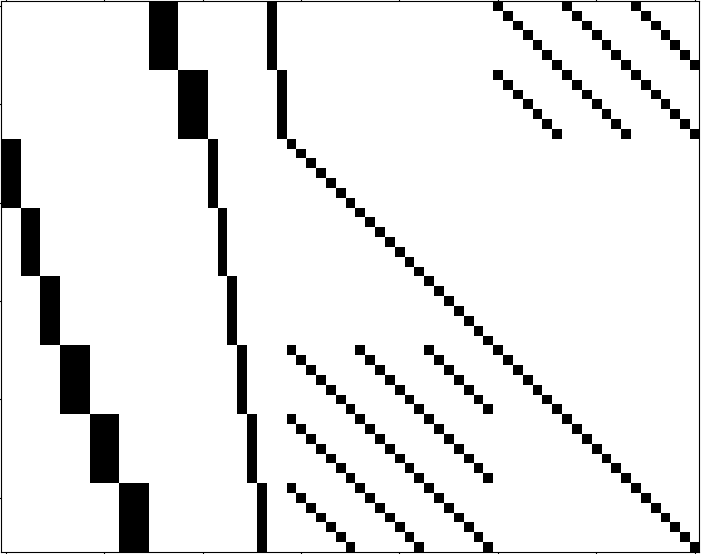
\includegraphics[width=\textwidth]{jac.png}
  \caption{Nonzero elements of jacobian, for network with I=2,O=2,W=3,D=2,N=7}
  \label{jac}
\end{figure}
How to read figure

\section{Algorithmic Verification of Jacobian}

\section{Alternative Representation}

In this section we explain an alternative representation which is mathematically the same.

